% Options for packages loaded elsewhere
\PassOptionsToPackage{unicode}{hyperref}
\PassOptionsToPackage{hyphens}{url}
%
\documentclass[
]{article}
\usepackage{lmodern}
\usepackage{amssymb,amsmath}
\usepackage{ifxetex,ifluatex}
\ifnum 0\ifxetex 1\fi\ifluatex 1\fi=0 % if pdftex
  \usepackage[T1]{fontenc}
  \usepackage[utf8]{inputenc}
  \usepackage{textcomp} % provide euro and other symbols
\else % if luatex or xetex
  \usepackage{unicode-math}
  \defaultfontfeatures{Scale=MatchLowercase}
  \defaultfontfeatures[\rmfamily]{Ligatures=TeX,Scale=1}
\fi
% Use upquote if available, for straight quotes in verbatim environments
\IfFileExists{upquote.sty}{\usepackage{upquote}}{}
\IfFileExists{microtype.sty}{% use microtype if available
  \usepackage[]{microtype}
  \UseMicrotypeSet[protrusion]{basicmath} % disable protrusion for tt fonts
}{}
\makeatletter
\@ifundefined{KOMAClassName}{% if non-KOMA class
  \IfFileExists{parskip.sty}{%
    \usepackage{parskip}
  }{% else
    \setlength{\parindent}{0pt}
    \setlength{\parskip}{6pt plus 2pt minus 1pt}}
}{% if KOMA class
  \KOMAoptions{parskip=half}}
\makeatother
\usepackage{xcolor}
\IfFileExists{xurl.sty}{\usepackage{xurl}}{} % add URL line breaks if available
\IfFileExists{bookmark.sty}{\usepackage{bookmark}}{\usepackage{hyperref}}
\hypersetup{
  hidelinks,
  pdfcreator={LaTeX via pandoc}}
\urlstyle{same} % disable monospaced font for URLs
\usepackage[margin=1in]{geometry}
\usepackage{graphicx,grffile}
\makeatletter
\def\maxwidth{\ifdim\Gin@nat@width>\linewidth\linewidth\else\Gin@nat@width\fi}
\def\maxheight{\ifdim\Gin@nat@height>\textheight\textheight\else\Gin@nat@height\fi}
\makeatother
% Scale images if necessary, so that they will not overflow the page
% margins by default, and it is still possible to overwrite the defaults
% using explicit options in \includegraphics[width, height, ...]{}
\setkeys{Gin}{width=\maxwidth,height=\maxheight,keepaspectratio}
% Set default figure placement to htbp
\makeatletter
\def\fps@figure{htbp}
\makeatother
\setlength{\emergencystretch}{3em} % prevent overfull lines
\providecommand{\tightlist}{%
  \setlength{\itemsep}{0pt}\setlength{\parskip}{0pt}}
\setcounter{secnumdepth}{-\maxdimen} % remove section numbering

\author{}
\date{\vspace{-2.5em}}

\begin{document}

\hypertarget{supporting-information-for-estimates-of-phylogenetic-signal-based-on-lambda-are-often-inaccurate}{%
\section{Supporting Information for: Estimates of Phylogenetic Signal
Based on Lambda are Often
Inaccurate}\label{supporting-information-for-estimates-of-phylogenetic-signal-based-on-lambda-are-often-inaccurate}}

Here we provide additional supporting information referenced in the main
document: additional analyses, and simulation results across a wider set
of input conditions.

\hypertarget{simulations-on-differently-shaped-phylogenies}{%
\subsection{Simulations on differently shaped
phylogenies}\label{simulations-on-differently-shaped-phylogenies}}

In addition to using pure-birth phylogenies, we explored the effect of
tree shape on our findings using both balanced and pectinate trees. As
before, simulations were conducted on a range of tree sizes
(\(n=2^5 - 2^{10}\)), and across a range of input levels of phylogenetic
signal (\(\lambda_{in} = 0.0 - 1.0\); in 21 intervals of 0.05 units).
For each \(n\) and \(\lambda_{in}\) combination, 50 replicates of a
continuous trait were simulated using a Brownian motion model of
evolution. Using these, we estimated the degree of phylogenetic signal
using \(\lambda\). \hfill\break

\emph{Results}. As found with pure-birth phylogenies, estimates of
\(\lambda\) varied \ldots.. ** FINISH THIS** (Fig. S1, S2).

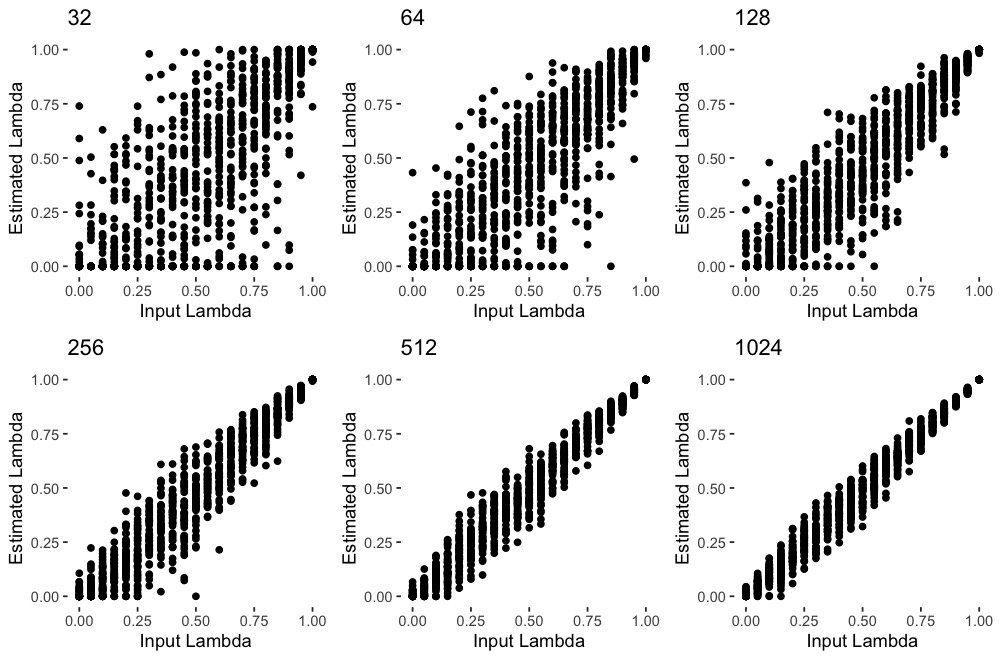
\includegraphics[width=0.75\linewidth]{Fig1}

\textbf{Figure S1}. Accuracy of Pagel's lambda estimations across known
lambda inputs on various tree sizes. Results obtained using balanced
trees. \hfill\break

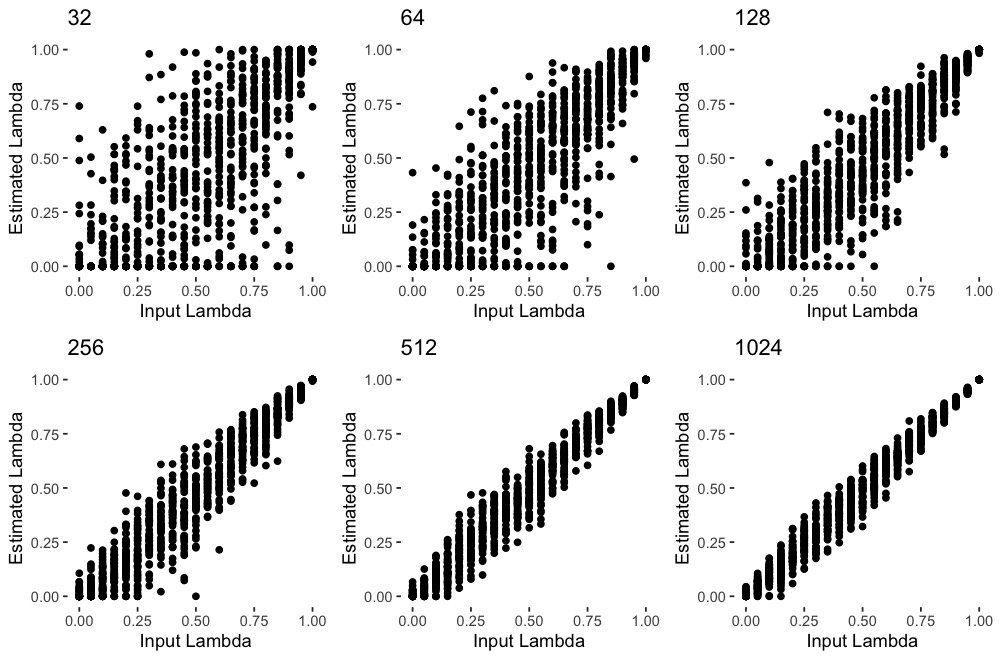
\includegraphics[width=0.75\linewidth]{Fig1}

\textbf{Figure S2}. Accuracy of Pagel's lambda estimations across known
lambda inputs on various tree sizes. Results obtained using pectinate
trees. \hfill\break

\hypertarget{literature-survey}{%
\subsection{Literature Survey}\label{literature-survey}}

\newpage

\hypertarget{references}{%
\section{References}\label{references}}

\setlength{\parindent}{-0.25in} \setlength{\leftskip}{0.25in}
\setlength{\parskip}{8pt} \noindent

\hypertarget{refs}{}

\end{document}
